\section {Central infrastructure}

CMS space monitoring central infrastructure is integrated into CMS central computing services 
supported by CMS computing operations and CERN IT division.
Historically, SpaceMon project stemmed from PhEDEx project for CMS data transfer infrastructure
\cite{phedex} and inherited many of PhEDEx developed solutions: Data Service interface to oracle database
\cite{dataservice} and security model. Authenticated write access to the information store for a given site 
is based on the individual's certificate and role registered in the CMS SiteDB \cite{sitedb} for that site.

Any CMS user with valid certificate can retrieve space usage information via Data Service 
{\it storageusage} API. The data directory paths are organized by level of depth and are available in 
perl. xml, or json formats. 

Another component of the SpaceMon central infrastructure currently in development is 
visualization of space monitoring data.  The goal of visualization is to present information 
in a convenient form, enabling users to check space usage across the sites, 
explore historical views or drill down into a particular directory in the   
CMS storage namespace. 
While this functionality is intented primarily for CMS computing management and the central data 
operations, it will likely become handy also for the site administrators and individual storage users.
After trying several prototypes, we opted for WLCG Experiment Dashboard \cite{ExpDashboard} 
framework for the space monitoring visualization. CMS dashboard, based on this 
framework, already provides visualization for monitoring job processing, data 
transfers and site/service usability.

Recently started work with WLCG dashboard developers resulted in the architecture 
proposal shown in Figure 2.
\begin{figure}[h]
\center
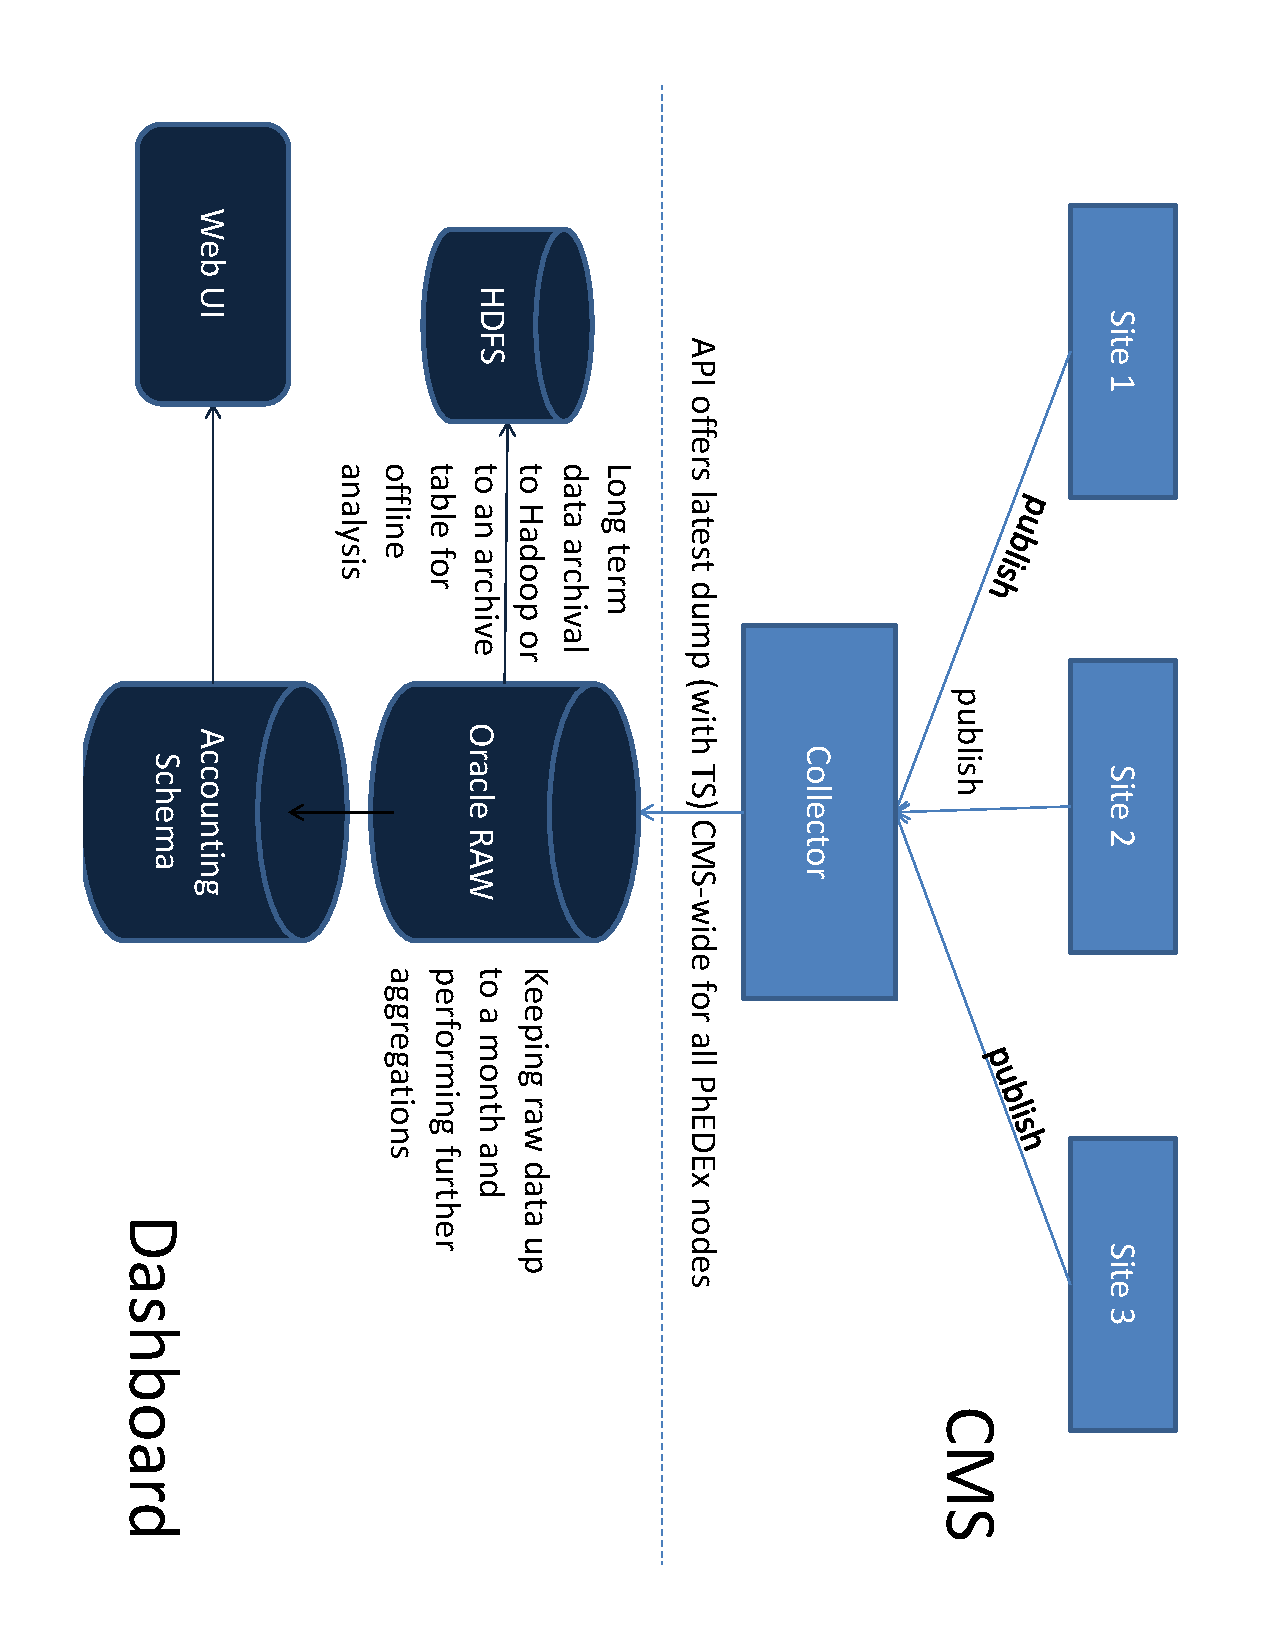
\includegraphics[width=0.8\linewidth, angle =90]
 {pictures/SpaceMonVisProposal-p1.pdf}    
\caption{Proposed architecture for storage accounting and visualization 
in CMS Dashboard based on CMS Space Monitoring information}
\label{fig:vis_proposal}
\end{figure}

Similar design was developed and deployed for ATLAS storage accounting \cite{DDMAccounting}
based on storage summaries from the central data management catalogs. The challenge in CMS 
case is to represent uniformly the monitoring data asynchronously pushed by the sites.
